\documentclass{article}
\usepackage[a4paper,landscape,margin=16mm]{geometry}
\usepackage{graphicx,booktabs,hyperref}
\begin{document}
\section*{S14160-1315PS + TPB: E/P pilot}
100 matched bb0nu events (IDs 0--99), 1 mm MC stepping, each gas and E/P point; 15 bar, 15\% He. Centred 1.3 $\times$ 1.3 mm S14160-1315PS at zero gap, 5 mm hole diameter/depth, 10 mm pitch. Uniform isotropic axial EL emission; absorbing surroundings. TPB coats the sensor; complete VUV absorption, intrinsic conversion 0.62, forward fraction 0.5, blue PDE approximated by its 0.32 peak: effective PDE 0.0992. Prompt TPB stays in the parent bucket. 7,284 cells, gain 360,000, dark rate 120 kHz. Provisional recharge 12.5 ns with approved 25 ns sensitivity; uniform microcell illumination and constant PDE during recovery. ASIC: 1 mA, 250 ns, 3.5417 PE RMS (same input charge noise as the previous sensor). J = 0.030 at E/P = 2.0 and 0.015 at 2.5, for both gases. Nominal results use 1024 statistical substeps per 250 ns bucket.
\begin{center}\small\begin{tabular}{lllllll}\toprule
E/P & Gas & Mean detected PE [million] & Sensor / detected [\%] & ASIC charge lost [\%] & Events clipping [\%] & Positive cells clipping [\%]\\\midrule
2.0 & Xe & 0.933 & 99.43 & 1.284 & 25 & 0.095\\
2.0 & Xe/He & 0.895 & 98.70 & 3.367 & 58 & 0.591\\
2.5 & Xe & 1.301 & 99.13 & 2.276 & 30 & 0.215\\
2.5 & Xe/He & 1.268 & 98.15 & 6.248 & 97 & 1.423\\
\bottomrule\end{tabular}\end{center}
Widths are full-distribution RMS/mean. Known attachment is corrected event by event and totals are divided by the deposited MC energy; sensor/ASIC sums have expected stationary dark baseline subtracted. Recovery and clipping remain in the forward response. The detected-PE width isolates optical counting statistics; the sensor and ASIC widths expose nonlinear response. These are not resolutions after a fitted nonlinearity correction. The raw total distributions also include energy deposition and drift variation. Each pulse is one SiPM--250 ns cell. The logarithmic pulse plot displays positive sensor output; zero outputs remain in all event sums and pulse means.
\begin{center}\small\begin{tabular}{llllll}\toprule
E/P & Gas & VUV RMS [\%] & Detected PE RMS [\%] & Sensor RMS [\%] & ASIC RMS [\%]\\\midrule
2.0 & Xe & 0.141 & 0.170 & 0.732 & 4.520\\
2.0 & Xe/He & 0.139 & 0.175 & 0.877 & 6.784\\
2.5 & Xe & 0.139 & 0.165 & 0.986 & 6.645\\
2.5 & Xe/He & 0.141 & 0.169 & 1.212 & 9.804\\
\bottomrule\end{tabular}\end{center}\clearpage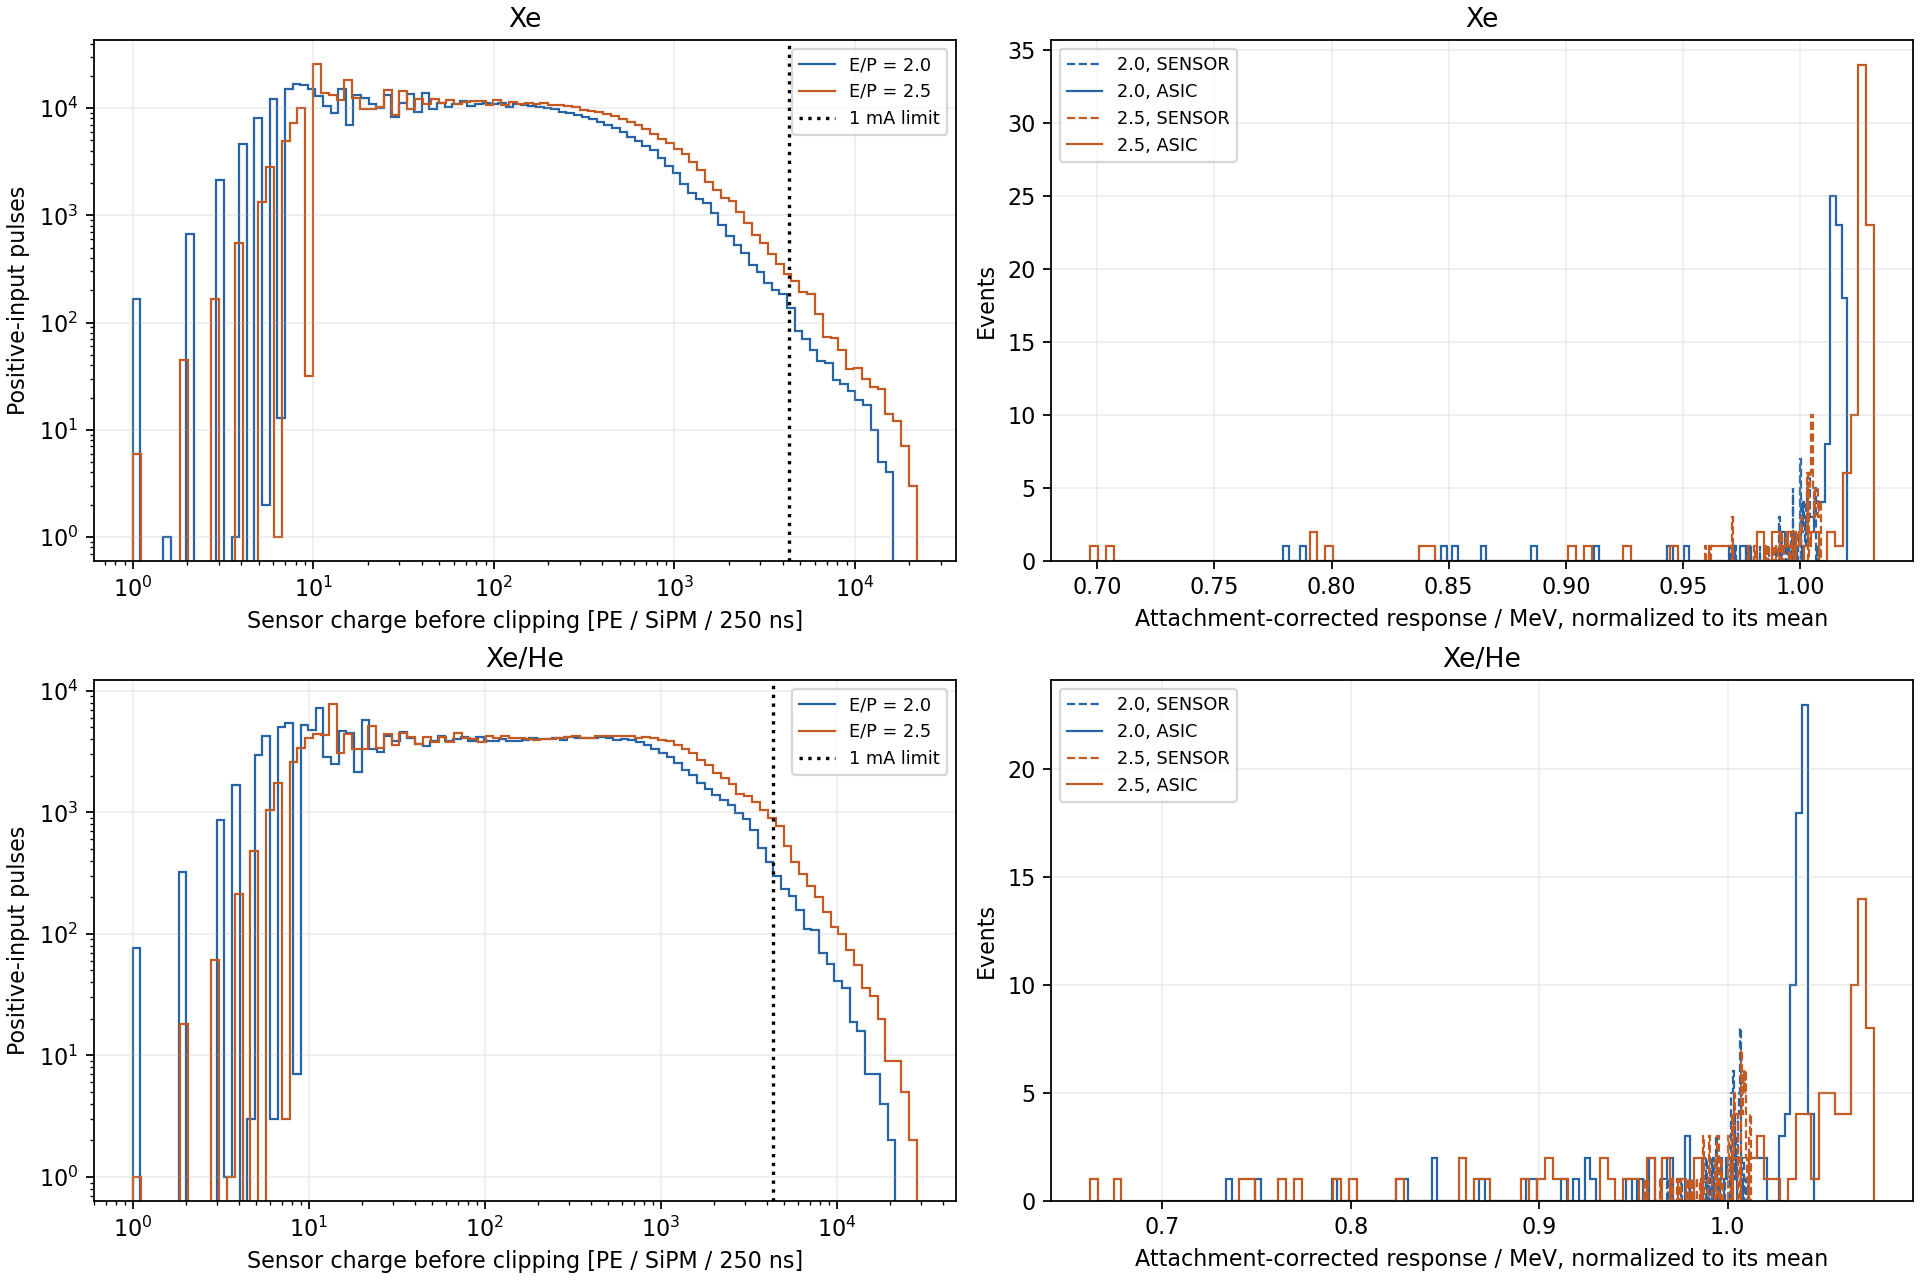
\includegraphics[width=\textwidth,height=.88\textheight,keepaspectratio]{tpb_response.png}\clearpage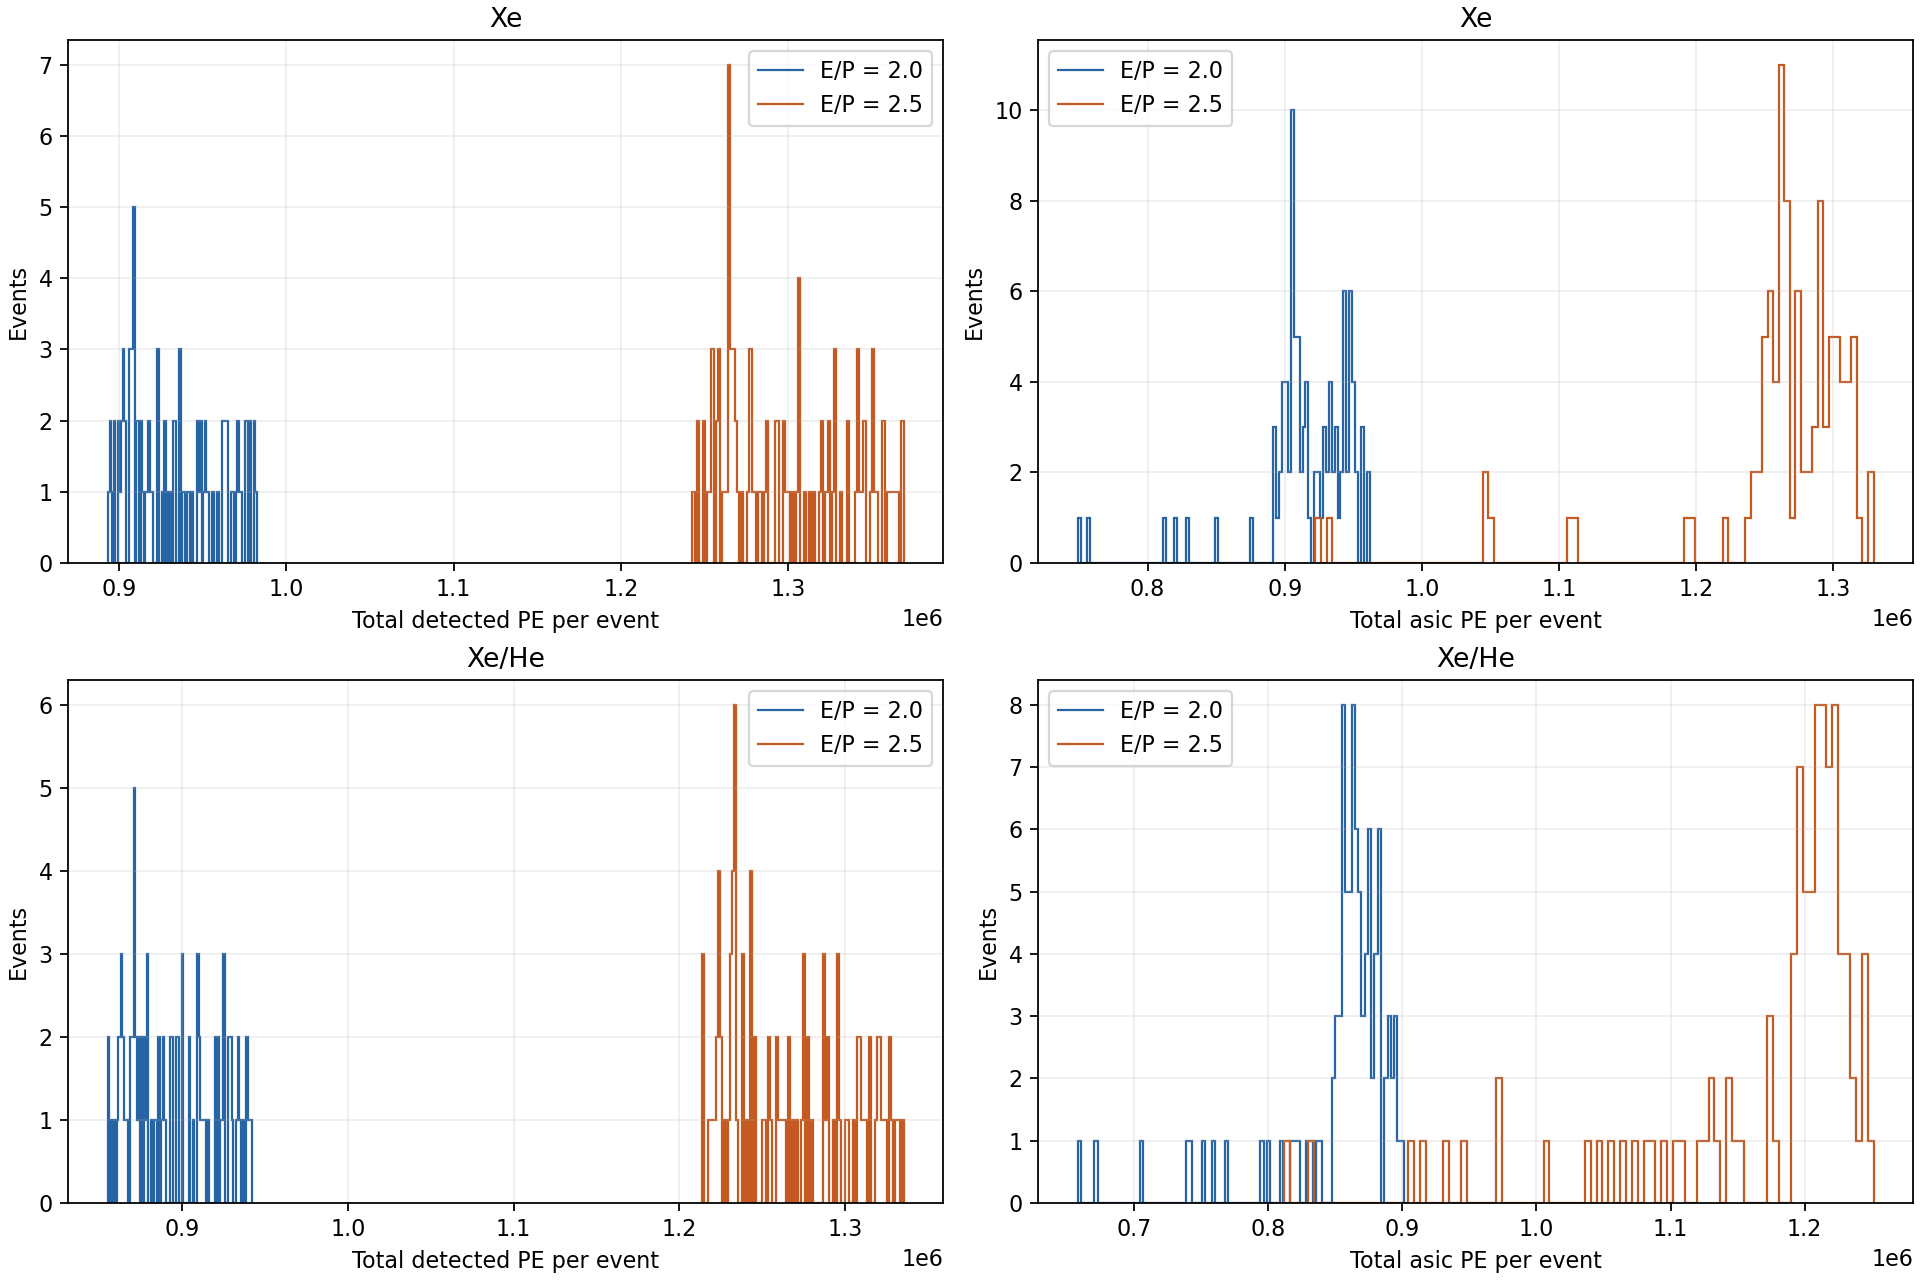
\includegraphics[width=\textwidth,height=.88\textheight,keepaspectratio]{tpb_totals.png}\clearpage\section*{Pulse and sensitivity summaries}\begin{center}\small\begin{tabular}{llllll}\toprule
E/P & Gas & Event-mean PE: mean & Event-mean PE: median & Event-max PE: mean & Event-max PE: median\\\midrule
2.0 & Xe & 250.8 & 155.0 & 3412.9 & 2054.6\\
2.0 & Xe/He & 493.5 & 351.9 & 6241.6 & 4562.5\\
2.5 & Xe & 347.8 & 215.5 & 4679.8 & 2842.0\\
2.5 & Xe/He & 693.6 & 495.3 & 8640.5 & 6346.1\\
\bottomrule\end{tabular}\end{center}\begin{center}\small\begin{tabular}{llllll}\toprule
Recharge ns / steps & E/P & Gas & ASIC loss [\%] & Sensor RMS [\%] & ASIC RMS [\%]\\\midrule
12.5 / 512 & 2.0 & Xe & 1.282 & 0.719 & 4.503\\
12.5 / 1024 & 2.0 & Xe & 1.284 & 0.732 & 4.520\\
25.0 / 512 & 2.0 & Xe & 1.116 & 1.372 & 4.663\\
12.5 / 512 & 2.0 & Xe/He & 3.365 & 0.878 & 6.775\\
12.5 / 1024 & 2.0 & Xe/He & 3.367 & 0.877 & 6.784\\
25.0 / 512 & 2.0 & Xe/He & 2.932 & 1.670 & 6.853\\
12.5 / 512 & 2.5 & Xe & 2.272 & 0.998 & 6.650\\
12.5 / 1024 & 2.5 & Xe & 2.276 & 0.986 & 6.645\\
25.0 / 512 & 2.5 & Xe & 1.973 & 1.855 & 6.779\\
12.5 / 512 & 2.5 & Xe/He & 6.242 & 1.220 & 9.806\\
12.5 / 1024 & 2.5 & Xe/He & 6.248 & 1.212 & 9.804\\
25.0 / 512 & 2.5 & Xe/He & 5.449 & 2.249 & 9.826\\
\bottomrule\end{tabular}\end{center}\begin{center}\small\begin{tabular}{llll}\toprule
E/P & Gas & Mean sensor change [\%] & Clip loss change [percentage points]\\\midrule
2.0 & Xe & +0.0036 & +0.0012\\
2.0 & Xe/He & -0.0012 & +0.0016\\
2.5 & Xe & -0.0107 & +0.0039\\
2.5 & Xe/He & -0.0090 & +0.0057\\
\bottomrule\end{tabular}\end{center}\section*{Physical references}
\begin{itemize}
\item \href{https://doi.org/10.1140/epjc/s10052-018-5807-z}{Benson et al. (2018), intrinsic TPB QE, Figure 19}
\item \href{https://www.hamamatsu.com/content/dam/hamamatsu-photonics/sites/documents/99_SALES_LIBRARY/ssd/s14160-1310ps_etc_kapd1070e.pdf}{Hamamatsu S14160 datasheet}
\item \href{https://indico.bnl.gov/event/20473/contributions/84622/attachments/51960/88885/BIC%2520SiPM%2520Choice%2520Intro.pdf}{Klest and Zurek, measured pulse decay, slide 16}\end{itemize}\end{document}